\documentclass[12pt, twoside]{article}
\usepackage[letterpaper, margin=1in, headsep=0.5in]{geometry}
\usepackage[english]{babel}
\usepackage[utf8]{inputenc}
\usepackage{amsmath}
\usepackage{amsfonts}
\usepackage{amssymb}
\usepackage{tikz}
\usetikzlibrary{quotes, angles}
\usepackage{graphicx}
%\usepackage{pgfplots}
%\pgfplotsset{width=10cm,compat=1.9}
%\usepgfplotslibrary{statistics}
%\usepackage{pgfplotstable}
%\usepackage{tkz-fct}
%\usepackage{venndiagram}

\usepackage{fancyhdr}
\pagestyle{fancy}
\fancyhf{}
\renewcommand{\headrulewidth}{0pt} % disable the underline of the header

\fancyhead[RE]{\thepage}
\fancyhead[RO]{\thepage \\ Name: \hspace{3cm}}
\fancyhead[L]{BECA / Dr. Huson / Geometry 10th Grade\\* Unit 3: Volume and angle bisectors  \\ 
7 October 2019}

\begin{document}
  \subsubsection*{3.3 Homework: Segment \& Area Calculations}
  \begin{enumerate}

  \item Complete the construction of the bisector of the given angle. 
  \vspace{3cm}
    \begin{center}
    \begin{tikzpicture}
      \draw [<->, thick] (1200:7)--(0,0)--(9,0);
      %\draw [fill] (0,0) circle [radius=0.05] node[below]{$A$};
      %\draw [fill] (5,0) circle [radius=0.05] node[below]{$B$};
    \end{tikzpicture}
    \end{center} \vspace{3cm}

  \item Find the area of the parallelogram $ABCD$ shown below, with $AB=12.2$ and height $h=5.8$.
    \begin{flushright}
    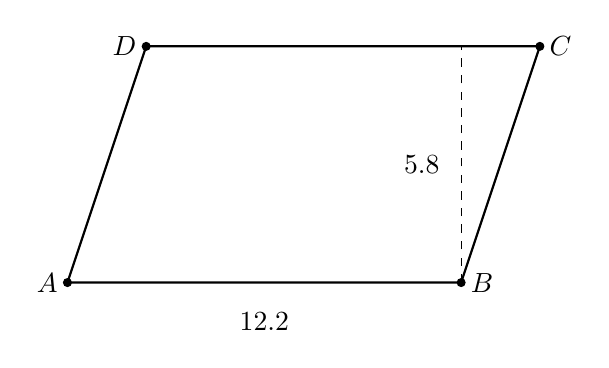
\begin{tikzpicture}[scale=1]
      \draw [-, thick] (0,0)--(5,0)--(6,3)--(1,3)--cycle;
      \draw [-, dashed] (5,0)--(5,3);
      \draw [fill] (0,0) circle [radius=0.05] node[left]{$A$};
      \draw [fill] (5,0) circle [radius=0.05] node[right]{$B$};
      \draw [fill] (6,3) circle [radius=0.05] node[right]{$C$};
      \draw [fill] (1,3) circle [radius=0.05] node[left]{$D$};
      \node at (4.5, 1.5){$5.8$};
      \node at (2.5, -0.5){12.2};
    \end{tikzpicture}
    \end{flushright}

\newpage
  \item The volume of a cube is 27 cubic inches. 
    \begin{enumerate}
      \item Find the length of the side of the cube, $s$. \vspace{2cm}
      \item Find the area of one face of the cube.
    \end{enumerate} \vspace{2cm}

  \item Given $\overleftrightarrow{FG}$ as shown on the number line, with $F=-3.1$ and $G=4.3$. \\[20pt] % Midpoint
  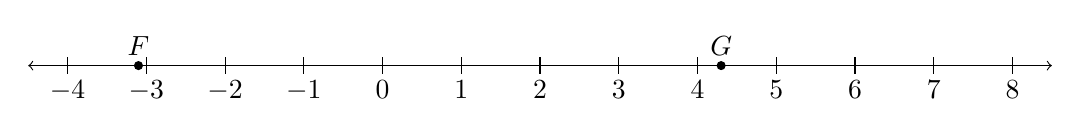
\begin{tikzpicture}
    \draw [<->] (-4.5,0)--(8.5,0);
    \foreach \x in {-4,...,8} %2 leading for diff!=1
      \draw[shift={(\x,0)},color=black] (0pt,-3pt) -- (0pt,3pt) node[below=5pt]  {$\x$};
      \draw [fill] (-3.1,0) circle [radius=0.05] node[above] {$F$};
      \draw [fill] (4.3,0) circle [radius=0.05] node[above] {$G$};
  \end{tikzpicture}\\[5pt]
  The point $H$ is the bisector of $\overline{FG}$. Find the value of $H$, and mark and label it on the numberline $\overleftrightarrow{FG}$ above. 
  \vspace{3cm}

  \item Given that $m\angle 1= 1x+30$ and $m\angle 4=6x+10$ as shown in the diagram, find $m\angle 2$.
  \begin{flushright}
  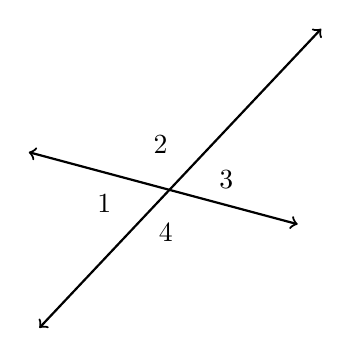
\begin{tikzpicture}[scale=0.5, rotate=30]
    \draw [<->, thick] (0,-1.5)--(10,1.5);
    \draw [<->, thick] (2,2.5)--(7,-2.5);
    \node at (3,.4){1};
    \node at (6,-.6){3};
    \node at (5,1){2};
    \node at (4,-1){4};
  \end{tikzpicture}
  \end{flushright}

\end{enumerate}
\end{document}
